\subsection{Setting and assumptions}
\label{assumptions}
As a preliminary step to the analysis of algorithm \ref{FedAVG}, we make the following 7 assumptions:

\begin{enumerate}
    \item At any round $t$ each \textit{client} takes $\tau \in \mathbb{N}$ local SGD steps with constant learning rate $\eta$ (which we denote as $\bm{x}_i^{(t,k+1)} \leftarrow \bm{x}_i^{(t,k)} - \eta g_i(\bm{x}_i^{(t,k)})$ with $g_i$ is one draw of the stochastic gradient of $F_i$ and $k \in [0,\tau)$.
    \item The \textit{server step} is computed as $\bm{x}^{(t+1)} \leftarrow \bm{x}^{(t)} + \Delta^{(t)}$.
    \item There are $(M)$ clients labelled $i \in \{0,1,...,M\}$ and each client contributes a uniform share of the global objective $F(\bm{x}) = \frac{1}{M} \sum^{M}_{i=1} F_i(\bm{x})$.
    \item Each clients takes part in every round.
    \item Each local objective $F_i$ is convex and $L$-smooth.
    \item Each client queries an unbiased stochastic gradient with $\sigma^2$-uniformly bounded variance in $l_2$ norm, i.e.
    \begin{align}
        \mathbb{E}[g_i(\bm{x}^{(t,k)}_i) | \bm{x}^{(t,k)}_i] = \nabla F_i(\bm{x}_i^{(t,j)}), \\
        \mathbb{E}[\| g_i(\bm{x}^{(t,k)}_i) -  F_i(\bm{x}_i^{(t,j)}) \|^2 | \bm{x}_i^{(t,k)} ] \leq \sigma^2.
    \end{align}
    \item The difference of local gradient $\nabla F_i(\bm{x})$ and the global gradient $\nabla F(\bm{x})$ is $\zeta$-uniformly bounded in $l_2$ norm, i.e.
    \begin{align}
        \max_i \sum_{\bm{x}} \| \nabla F_i(\bm{x}) - \nabla F(\bm{x}) \| \leq \zeta.
    \end{align}
\end{enumerate}

First, let us define the shadow sequence which we will use to make the notation a bit more readable as we go through the proof:

\begin{notation}
    (Shadow sequence) We call the sequence described by $\bar{x}^{t,k} = \frac{1}{M} \sum_{i=1}^{M} \bm{x}_i^{(t,k)}$ the shadow sequence.
\end{notation}

As we often do in the optimization literature we will try to show a result of the form: 
\[ \mathbb{E}\left[ \frac{1}{\tau T} \sum_{t=0}^{T-1} \sum_{k=1}^{\tau} F(\bar{\bm{x}}^{(t,k)}) -F(\bm{x}^*) \right] = O\left( \frac{1}{\tau T} \right). \]

Which one can read as \textit{as we progress, in expectation we are guaranteed to have an error that goes to some small constant}. In order to get to a bound we will have to prove two lemmas to show that. Showing that this results is true amounts to finding a relevant upper bound decreasing in $\frac{1}{\tau T}$. We split our proving effort in two steps:


\begin{enumerate}
    \item We are making progress in each round $\mathbb{E}\left[ \frac{1}{\tau} \sum^{\tau}_{k=1} F(\bar{\bm{x}}^{(t,k)}) - F(\bm{x}^*) \right]$ is bounded by some term decreasing when $t$ increases.
    \item All client iterates remain close to the global average (the shadow sequence), i.e. $\| \bm{x}_i^{(t,k)} - \hat{\bm{x}}^{(t,k)}  \|_{l_2}$ is bounded in expectation.
\end{enumerate}

Formally we will write our proof using one theorem that relies on two lemmas (showing both properties discussed above). The formal proofs are detailed in the next section.

\begin{figure}[h!]
    \centering
    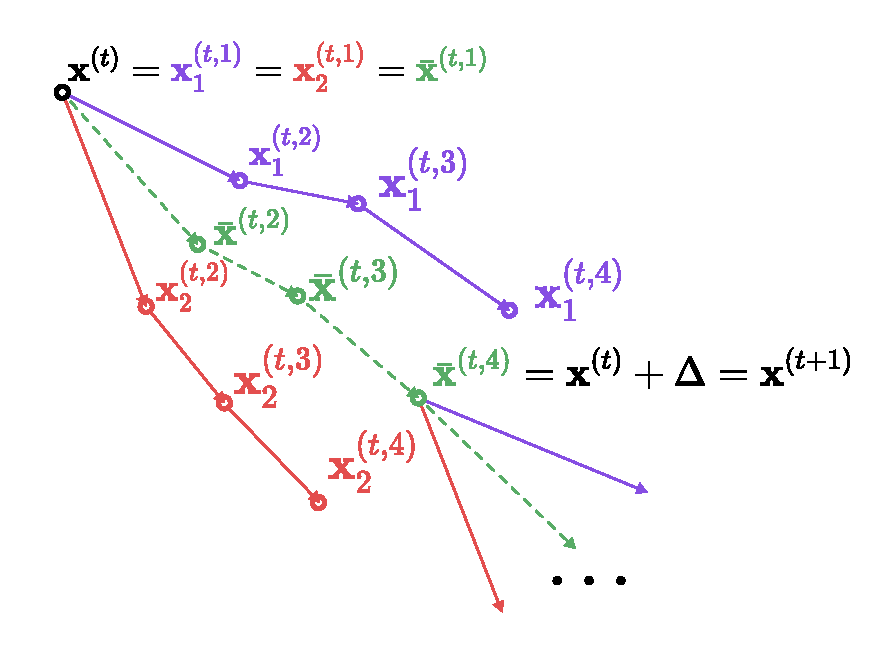
\includegraphics[width=0.6\textwidth]{figures/FedAVG_traj.pdf}
    \caption{Illustration of the progression of one $4$ step round of algorithm \ref{FedAVG} with the shadow sequence represented on green.}
\end{figure}

\subsection{Convergence of FedAVG}

We will prove the following results. 


\begin{theorem}
    (Convergence for Convex Functions) under the assumptions and assuming $\eta \leq \frac{1}{4L}$ one has: 

    \begin{equation}
        \begin{aligned}
            \mathbb{E} \left[ \frac{1}{\tau T} \sum_{t=0}^{T-1}\sum_{k=1}^{\tau} F(\bar{\bm{x}}^{(t,k)}) - F(\bm{x}^*)\right] 
            \leq \frac{D^2}{2 \eta \tau T} + \frac{\eta \sigma^2}{M} + 4 \tau \eta^2 L \sigma^2 + 18 \tau^2 \eta^2 L \zeta^2 \\
            = O\left( \frac{1}{\tau T} \right)
        \end{aligned}
        \label{eq:convergence}
    \end{equation}
    \label{convergence}
\end{theorem}

\noindent
To which we will get using two lemmas:

\begin{lemma}
    (Per round progress) Assuming $\eta \leq \frac{1}{4L}$, for one round $t$ of the algorithm, one has: 
    
    \begin{equation}
        \begin{aligned}
            \mathbb{E} \left[ \frac{1}{\tau} \sum_{k=1}^{\tau} F(\bar{\bm{x}}^{(t,k)}) - F(\bm{x}^*)\right]  \\
            \leq \frac{1}{2 \eta \tau} \left( \| \bar{\bm{x}}^{(t,0)} -\bm{x}^{*} \|^2 - \mathbb{E}\left[  \| \bar{\bm{x}}^{(t,\tau)} -\bm{x}^{*} \|^2  | \mathcal{F}^{(t,0)}\right]  \right)\\
            + \frac{\eta \sigma^2}{M} + \overbrace{\frac{1}{M \tau} \sum^M_{i=1} \sum^{\tau-1}_{k=1} \mathbb{E} \left[ \| \bm{x}_i^{(t,k)} -\bar{\bm{x}}^{(t,k)} \|^2 | \mathcal{F}^{(0,t)}\right]}^\text{client drift}
        \end{aligned}
        \label{eq:per_round_progress}
    \end{equation}
    \label{per_round_progress}
\end{lemma}

\begin{lemma}
    (Bounded client drift) Assuming $\eta \leq \frac{1}{4L}$, for one round $t$ of the algorithm, one has: 
    
    \begin{equation}
        \begin{aligned}
            \mathbb{E} \left[ \| \bm{x}_i^{(t,k)} -\bar{\bm{x}}^{(t,k)} \|^2 | \mathcal{F}^{(0,t)}\right]
            \leq 18\tau^2 \eta^2 \zeta^2 + 4 \tau \eta^2 \sigma^2
        \end{aligned}
        \label{eq:client_drift}
    \end{equation}
    \label{client_drift}
\end{lemma}

\subsubsection*{Proving Theorem \ref{convergence} (convergence of FedAVG)}

Most of the technical work will lie in proving the two lemmas, but first we will focus on proving theorem \ref{convergence}, while assuming that lemmas \ref{per_round_progress} and \ref{client_drift} are true.

\begin{proof}
    (Of Theorem \ref{convergence}.) We want to find a bound for the quantity \[ \mathbb{E} \left[ \frac{1}{\tau T} \sum_{t=0}^{T-1}\sum_{k=1}^{\tau} F(\bar{\bm{x}}^{(t,k)}) - F(\bm{x}^*)\right], \]
    to do so we will use the bound on $\mathbb{E} \left[ \frac{1}{\tau} \sum_{k=1}^{\tau} F(\bar{\bm{x}}^{(t,k)}) - F(\bm{x}^*)\right]$ which is given by lemma \ref{per_round_progress}. First, let's write out the sum on which we will take the expectation and express it as a function of the per round client progress which we bounded in lemma \ref{per_round_progress}:

    \begin{align*}
        \mathbb{E} \left[ \frac{1}{\tau T} \sum_{t=0}^{T-1}\sum_{k=1}^{\tau} F(\bar{\bm{x}}^{(t,k)}) - F(\bm{x}^*)\right], \\
        = \mathbb{E} \left[\frac{1}{T} \sum^{T-1}_{t=0} \overbrace{\mathbb{E} \left[ \frac{1}{\tau} \sum_{k=1}^{\tau} F(\bar{\bm{x}}^{(t,k)}) - F(\bm{x}^*)\right] }^{(\triangledown)}\right].
    \end{align*}
    Observing that the term $(\triangledown)$ is the left side of the inequality (\ref{eq:per_round_progress}) of lemma \ref{per_round_progress}, we use the lemma to bound our expectation. Using linearity of expectation we split this expression in three different terms which we will then discuss separately.
    \begin{align*}
        (\triangledown) \leq \mathbb{E}
        \Bigg[ \frac{1}{T} \sum_{t=0}^{T-1} \frac{1}{2 \eta \tau} \left( \| \bar{\bm{x}}^{(t,0)} -\bm{x}^{*} \|^2 - \mathbb{E}\left[  \| \bar{\bm{x}}^{(t,\tau)} -\bm{x}^{*} \|^2  | \mathcal{F}^{(t,0)}\right]  \right) \\
        + \frac{\eta \sigma^2}{M} + \frac{1}{M \tau} \sum^M_{i=1} \sum^{\tau-1}_{k=1} \mathbb{E} \left[ \| \bm{x}_i^{(t,k)} -\bar{\bm{x}}^{(t,k)} \|^2 | \mathcal{F}^{(0,t)}\right] \Bigg] \\
        = \overbrace{\mathbb{E}\Bigg[ \frac{1}{T} \sum_{t=0}^{T-1} \frac{1}{2 \eta \tau} \left( \| \bar{\bm{x}}^{(t,0)} -\bm{x}^{*} \|^2 - \mathbb{E}\left[  \| \bar{\bm{x}}^{(t,\tau)} -\bm{x}^{*} \|^2  | \mathcal{F}^{(t,0)}\right] \right) \Bigg]}^{(\bigstar)} \\
        + \overbrace{\frac{\eta \sigma^2}{M}}^{(\diamond)} +  \overbrace{\frac{1}{M \tau}\sum^M_{i=1} \sum^{\tau-1}_{k=1} \mathbb{E} \left[ \| \bm{x}_i^{(t,k)} -\bar{\bm{x}}^{(t,k)} \|^2 | \mathcal{F}^{(0,t)}\right] }^{(\dagger)}
    \end{align*}
    Let us now consider the three terms. Terms $(\diamond)$ and $(\dagger)$ gives a bound on individual client drift (i.e. how far do the clients get from the shadow sequence), term $(\bigstar)$ gives a bound on the global progression. Here our goal is to show that $(\diamond)$ and $(\dagger)$ can be arbitrarily bounded as a function of the algorithm's parameters and that $(\bigstar)$ goes to $0$ with $T\cdot \tau$. We now discuss bounds for every single term.
    \begin{enumerate}
        \item Term $(\diamond)$ is already a function of our algorithm's parameters, there is nothing to show here.
        \item Now we consider term $(\dagger)$, this is the drift term:
        \[ \frac{1}{M \tau}\sum^M_{i=1} \sum^{\tau-1}_{k=1} \overbrace{\mathbb{E} \left[ \| \bm{x}_i^{(t,k)} -\bar{\bm{x}}^{(t,k)} \|^2 | \mathcal{F}^{(0,t)}\right]}^{(\spadesuit)} \]
        it is a sum over term $(\spadesuit)$, which is the left side the inequality (\ref{eq:client_drift}) of lemma \ref{client_drift}. We plug the right side of (\ref{eq:client_drift}) and as it is not a function of the sum variables we can drop the sums as well.
        \begin{align*}
            (\dagger) \leq 18\tau^2 \eta^2 \zeta^2 + 4 \tau \eta^2 \sigma^2 \\
        \end{align*}
        \item Finally we consider term $(\bigstar)$, 
        \begin{align*}
            \mathbb{E}\Bigg[ \frac{1}{T} \sum_{t=0}^{T-1} \frac{1}{2 \eta \tau} \left( \| \bar{\bm{x}}^{(t,0)} -\bm{x}^{*} \|^2 - \mathbb{E}\left[  \| \bar{\bm{x}}^{(t,\tau)} -\bm{x}^{*} \|^2  | \mathcal{F}^{(t,0)}\right] \right) \Bigg],
        \end{align*}
        here we have to use a few tricks. First using that expectation is linear we will separate our terms and using that $\mathbb{E}\left[ \mathbb{E}[x] \right] = \mathbb{E}[x]$ we will drop the double expectation in the sum:
        \begin{align*}
            \frac{1}{2 \eta \tau T}  \sum_{t=0}^{T-1}   \left(\mathbb{E}\left[  \| \overbrace{\bar{\bm{x}}^{(t,0)}}^{\bar{\bm{x}}^{(t)}} -\bm{x}^{*} \|^2 \right] - \mathbb{E}\left[  \| \overbrace{\bar{\bm{x}}^{(t,\tau)}}^{\bar{\bm{x}}^{(t+1)}} -\bm{x}^{*} \|^2  \right] \right).
        \end{align*}
        At this point we first observe (as denoted above) that by definition of the algorithm we have $\bar{\bm{x}}^{(t+1)} = \bar{\bm{x}}^{(t+1,0)} = \bar{\bm{x}}^{(t,\tau)}$ and $\bar{\bm{x}}^{(t)} = \bar{\bm{x}}^{(t,0)}$, then for readability we make use of the notation $d(\bm{x}) = \mathbb{E} \left[ \| \bm{x}-\bm{x}^*\|^2 \right]$ and write out the sum over $t$:
        \begin{align*}
           \sum_{t=0}^{T-1}  \left( d(\bm{x}^{(t)}) - d(\bm{x}^{(t+1)}) \right)
            \\=  d(\bm{x}^{(0)}) - d(\bm{x}^{(1)}) +  d(\bm{x}^{(1)}) - d(\bm{x}^{(2)})  \\
            + \cdots +  d(\bm{x}^{(T-2)}) - d(\bm{x}^{(T-1)})  + d(\bm{x}^{(T-1)}) - d(\bm{x}^{(T)}) .
        \end{align*}
        Observing that the terms cancel out we get the following expression: 
        \begin{align*}
        (\bigstar)= \frac{1}{2 \eta \tau T} \Big( d(\bm{x}^{(0)}) - \cancel{d(\bm{x}^{(1)})} +  \cancel{ d(\bm{x}^{(1)})} - \cancel{d(\bm{x}^{(2)})}  \\
        + \cdots + \cancel{ d(\bm{x}^{(T-2)}) } - \cancel{ d(\bm{x}^{(T-1)}) } + \cancel{ d(\bm{x}^{(T-1)}) } -  d(\bm{x}^{(T)}) \Big) \\= \frac{1}{2 \eta \tau T} \Big( d(\bm{x}^{(0)})  -  d(\bm{x}^{(T)}) \Big) \leq \frac{d(\bm{x}^{(0)})}{2 \eta \tau T} = \frac{D^2}{2 \eta \tau T} .
        \end{align*}
        Where $d(\bm{x}^{(0)}) = \mathbb{E}[\| \bm{x}^{(0)} -\bm{x}^* \|^2] = \| \bm{x}^{(0)} -\bm{x}^* \|^2 = D^2$ with $D$ the diameter to the global opt at the beginning of the gradient descent (this is a constant).
    \end{enumerate}
    Putting all bounds back together we get the following convergence bound (which concludes the proof):
    \[\mathbb{E} \left[ \frac{1}{\tau T} \sum_{t=0}^{T-1}\sum_{k=1}^{\tau} F(\bar{\bm{x}}^{(t,k)}) - F(\bm{x}^*)\right] 
    \leq \overbrace{\frac{D^2}{2 \eta \tau T} }^{(\bigstar)}+\overbrace{ \frac{\eta \sigma^2}{M}}^{(\diamond)} + \overbrace{4 \tau \eta^2 L \sigma^2 + 18 \tau^2 \eta^2 L \zeta^2}^{(\dagger)} \]
    
\end{proof}

We now get in the (somewhat) more technical parts of the proof, proving that both the lemmas are correct. 

\subsubsection*{Proving Lemma \ref{per_round_progress} (per round progression)}
\begin{proof}  (Of Lemma \ref{per_round_progress}.)\\
    
Let's start with the per round progress lemma, we want to bound the quantity : 

\begin{align*}
    \mathbb{E} \left[ \frac{1}{\tau} \sum_{k=1}^{\tau} F(\bar{\bm{x}}^{(t,k)}) - F(\bm{x}^*)\right],
\end{align*}

in $O(\frac{1}{\tau})$. Similarly to what we just did for the theorem (and to how most of these convergence proofs are computed), we will to try to bound a single term of the sum (in expectation) by the previous term and then we will telescope the sum to get a serviceable bound. In other words we are trying to bound the expectation:

\begin{align}
    (\dagger) = \mathbb{E} \Big[ \overbrace{F(\bar{\bm{x}}^{(t,k+1)}) - F(\bm{x}^*)}^{(\heartsuit)} | \mathcal{F}^{(t,k)}\Big],
    \label{eq:expected_sub_progress}
\end{align}

In order to get a bound on the expectation $(\dagger)$, most of the work we will have to do will lie in understanding the $(\heartsuit)$ term on which we take the expectation. \textit{This is where the proof starts getting technical}. Writing it out we can first split it between the separate client objective functions:

\begin{align}
    (\heartsuit) = F(\bar{\bm{x}}^{(t,k+1)}) - F(\bm{x}^*) = \frac{1}{M} \sum_{i=1}^M \left( F_i(\bar{\bm{x}}^{(t,k+1)})  - F(\bm{x}^*)\right).
    \label{eq:sub_progress}
\end{align}

\begin{figure}[h!]
    \centering
    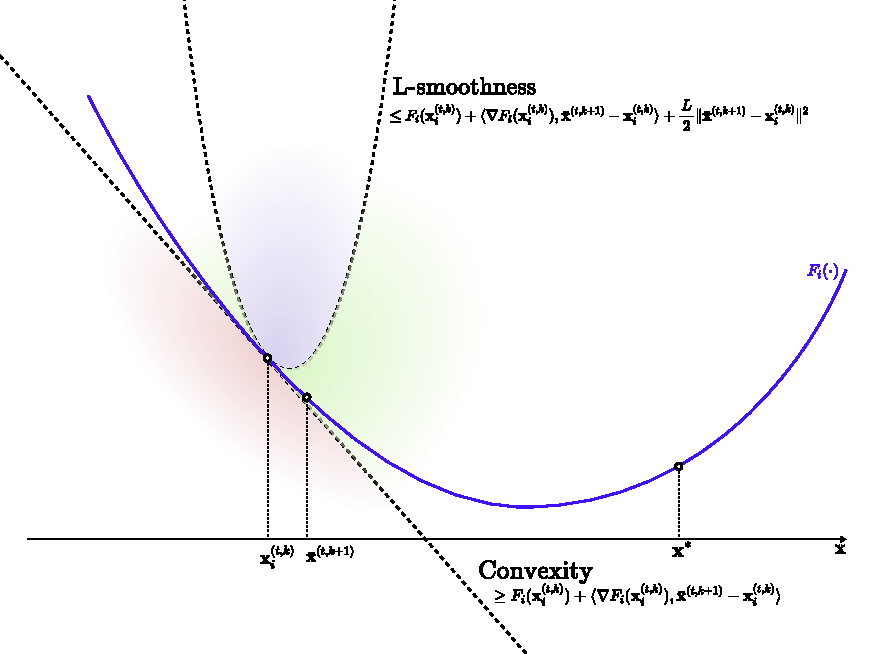
\includegraphics[width=0.6\textwidth]{figures/smooth_convex.pdf}
    \caption{Illustration of the L-smooth/convex properties of $F_i$. Convexity implies that the function is above the half space tangent to the graph at any point (in red) and that is is below the parabola with parameter $L$ (in blue). In other words, the function being L-smooth and convex is necessarily in the green area of the plot. Furthermore observe that the global minimum $\bm{x}^*$ of $F$ is not the minimum of $F_i$, so we cannot use that property directly.}
\end{figure}

Looking at the expression above, we clearly see that bounding $(\heartsuit)$ will amount to bound $F_i(\bar{\bm{x}}^{(t,k+1)})$, which we will do using the smoothness (property \ref{lsmooth}) and convexity (property \ref{convexity}) properties from the assumptions made in section \ref{assumptions}. First, we get an upper bound from the L-smoothness (property \ref{lsmooth}) of $F_i$:

\begin{align*}
    F_i(\bar{\bm{x}}^{(t,k+1)}) \leq  F_i(\bm{x}) +  \langle \nabla F_i(\bm{x}) ,\bar{\bm{x}}^{(t,k+1)}-\bm{x} \rangle +  \frac{L}{2} \|\bar{\bm{x}}^{(t,k+1)}-\bm{x} \|^2, ~ \forall \bm{x}.
\end{align*}

This inequality is true for all $\bm{x} \in \bm{dom}(f)$ but we care about the algorithm's step and for each $F_i(\bar{\bm{x}}^{(t,k+1)})$ the step of the algorithm depends of $\bm{x}_i^{(t,k)}$ (the parameters of client $i$ at the previous time step). Using observation \ref{obs} (which we can do as $F_i$ is convex) we further bound the $(\spadesuit)$ term as a function of $\bm{x}^*$ instead of $\bm{x}_i^{(t,k)}$ which we don't know.

\begin{align*}
    F_i(\bar{\bm{x}}^{(t,k+1)}) \leq \overbrace{F_i(\bm{x}_i^{(t,k)}) +  \langle \nabla F_i(\bm{x}_i^{(t,k)}) ,\bar{\bm{x}}^{(t,k+1)}-\bm{x}_i^{(t,k)} \rangle}^{(\spadesuit)} +  \frac{L}{2} \|\bar{\bm{x}}^{(t,k+1)}-\bm{x}_i^{(t,k)} \|^2 \\
    \leq F_i(\bm{x}^{*}) +  \langle \nabla F_i(\bm{x}_i^{(t,k)}) ,\bar{\bm{x}}^{(t,k+1)} - \bm{x}^{*} \rangle + \overbrace{ \frac{L}{2} \|\bar{\bm{x}}^{(t,k+1)}-\bm{x}_i^{(t,k)} \|^2}^{\square}
\end{align*}

Now in order to get a bound on the $(\square)$ term we will try to split the $\bm{x}_i^{(t,k)}$ variable and express our bound as a function of the  pre step progress and the distance between clients (which we will bound using the client drift lemma later). To do so we use the triangle inequality ($\|a+b\| \leq \|a\|+\|b\|$):


\begin{align*}
    \overbrace{\bar{\bm{x}}^{(t,k+1)}-\bm{x}_i^{(t,k)}}^{a+b} = \overbrace{\bar{\bm{x}}^{(t,k+1)} - \bar{\bm{x}}^{(t,k)}}^a + \overbrace{\bar{\bm{x}}^{(t,k)} - \bm{x}_i^{(t,k)} }^b\\
    \square = \frac{L}{2} \|\bar{\bm{x}}^{(t,k+1)}-\bm{x}_i^{(t,k)} \|^2 \\
    \leq  \frac{L}{2} \|\bar{\bm{x}}^{(t,k+1)}-\bar{\bm{x}}^{(t,k)} \|^2  + \frac{L}{2} \|\bar{\bm{x}}^{(t,k)}-\bm{x}_i^{(t,k)} \|^2  \\
    \leq  L \|\bar{\bm{x}}^{(t,k+1)}-\bar{\bm{x}}^{(t,k)} \|^2  + L \|\bar{\bm{x}}^{(t,k)}-\bm{x}_i^{(t,k)} \|^2 
\end{align*}

The last step is just done for readability, we could actually get a tighter bound by keeping the factor two in there. Plugging this back in the $F_i(\bar{\bm{x}}^{(t,k+1)})$ bound we get the following inequality:


\begin{align*}
    F_i(\bar{\bm{x}}^{(t,k+1)}) \leq F_i(\bm{x}^{*}) +  \langle \nabla F_i(\bm{x}_i^{(t,k)}) ,\bar{\bm{x}}^{(t,k+1)} - \bm{x}^{*} \rangle \\+ L \|\bar{\bm{x}}^{(t,k+1)}-\bar{\bm{x}}^{(t,k)} \|^2  + L \|\bar{\bm{x}}^{(t,k)}-\bm{x}_i^{(t,k)} \|^2 
\end{align*}

Let's plug what we just derived in equation (\ref{eq:sub_progress}):


\begin{align*}
    (\heartsuit) = F(\bar{\bm{x}}^{(t,k+1)}) - F(\bm{x}^*) = \frac{1}{M} \sum_{i=1}^M \left( F_i(\bar{\bm{x}}^{(t,k+1)})  - F(\bm{x}^*)\right) \\
    \leq  \frac{1}{M} \sum_{i=1}^M \Big( F_i(\bm{x}^{*}) +  \langle \nabla F_i(\bm{x}_i^{(t,k)}) ,\bar{\bm{x}}^{(t,k+1)} - \bm{x}^{*} \rangle \\+ L \|\bar{\bm{x}}^{(t,k+1)}-\bar{\bm{x}}^{(t,k)} \|^2  + L \|\bar{\bm{x}}^{(t,k)}-\bm{x}_i^{(t,k)} \|^2  - F(\bm{x}^*)\Big).
\end{align*}

Using the linearity of the sum we can split this expression into separate terms:

\begin{align*}
    (\heartsuit) \leq \overbrace{\frac{1}{M} \sum_{i=1}^M F_i(\bm{x}^{*}) - F(\bm{x}^*)}^{=0} + \frac{1}{M} \sum_{i=1}^M  \langle \nabla F_i(\bm{x}_i^{(t,k)}) ,\bar{\bm{x}}^{(t,k+1)} - \bm{x}^{*} \rangle \\+ L \frac{1}{M} \sum_{i=1}^M \overbrace{ \|\bar{\bm{x}}^{(t,k+1)}-\bar{\bm{x}}^{(t,k)} \|^2}^\text{not a function of $i$}  + L \frac{1}{M} \sum_{i=1}^M \|\bar{\bm{x}}^{(t,k)}-\bm{x}_i^{(t,k)} \|^2 \\
    = \overbrace{\frac{1}{M} \sum_{i=1}^M  \langle \nabla F_i(\bm{x}_i^{(t,k)}) ,\bar{\bm{x}}^{(t,k+1)} - \bm{x}^{*} \rangle}^{(\blacklozenge)} \\+ L  \|\bar{\bm{x}}^{(t,k+1)}-\bar{\bm{x}}^{(t,k)} \|^2  +\overbrace{ L \frac{1}{M} \sum_{i=1}^M \|\bar{\bm{x}}^{(t,k)}-\bm{x}_i^{(t,k)} \|^2 }^{{\blacksquare}}
\end{align*}

This brings us closer to bounding the $(\heartsuit)$ term, remembering that we are working with values inside of an expectation, we clearly see that term $(\blacksquare)$ is a measure of client drift (which we will bound later with the client drift lemma). Taking a look at the sum the term that requires and explanation is the $(\blacklozenge)$ term, which we will now take a look at. Recall that the FedAVG algorithm queries stochastic gradients $g_i$, which are unbiased, variance bounded estimators of the true gradient $\nabla F_i$. Observe that we can write out the local true client gradient as:

\begin{align}
    \nabla F_i(\bm{x}) = \overbrace{g_i(\bm{x})}^{(\triangleleft)} + \overbrace{\left(F_i(\bm{x}) - g_i(\bm{x}) \right)}^{(\triangleright)},
    \label{eq:grad_dev}
\end{align}

where $(\triangleleft)$ represents the sampled gradient of client objective $F_i$ (which is used for gradient descent steps) and $(\triangleright)$ the deviation from the true gradient value value. This is useful as we know from the assumptions that the deviation is $0$ in expectation ($g_i$ is an unbiased estimator of $\nabla F_i$). Using the decomposition (\ref{eq:grad_dev}) we can develop the $(\heartsuit)$ bound as follows:

\begin{align*}
    (\heartsuit) \leq \frac{1}{M} \sum_{i=1}^M  \langle g_i(\bm{x})  + \left(F_i(\bm{x}) - g_i(\bm{x}) \right) ,\bar{\bm{x}}^{(t,k+1)} - \bm{x}^{*} \rangle  \\+ L  \|\bar{\bm{x}}^{(t,k+1)}-\bar{\bm{x}}^{(t,k)} \|^2  +L \frac{1}{M} \sum_{i=1}^M \|\bar{\bm{x}}^{(t,k)}-\bm{x}_i^{(t,k)} \|^2 \\
    = \overbrace{\frac{1}{M} \sum_{i=1}^M  \langle g_i(\bm{x})  ,\bar{\bm{x}}^{(t,k+1)} - \bm{x}^{*} \rangle  }^{(\blacktriangleleft)}
    + \overbrace{\frac{1}{M} \sum_{i=1}^M  \langle F_i(\bm{x}) - g_i(\bm{x})  ,\bar{\bm{x}}^{(t,k+1)} - \bm{x}^{*} \rangle  }^{(\blacktriangleright)}
    \\+ L  \|\bar{\bm{x}}^{(t,k+1)}-\bar{\bm{x}}^{(t,k)} \|^2  +L \frac{1}{M} \sum_{i=1}^M \|\bar{\bm{x}}^{(t,k)}-\bm{x}_i^{(t,k)} \|^2 
\end{align*}

We will analyze $(\blacktriangleright)$ later, when we take expectations, let us now focus on $(\blacktriangleleft)$. Using that client algorithm steps are computed as $\bm{x}_i^{(t,k+1)} = \bm{x}_i^{(t,k)} - \eta g_i(\bm{x}_i^{(t,k)})$, and that the inner product is distributive over addition we can develop $(\blacktriangleleft)$ as follows:

\begin{align*}
    (\blacktriangleleft) = \frac{1}{M} \sum_{i=1}^M  \langle g_i(\bm{x})  ,\bar{\bm{x}}^{(t,k+1)} - \bm{x}^{*} \rangle =  \langle \frac{1}{M} \sum_{i=1}^M  g_i(\bm{x})  ,\bar{\bm{x}}^{(t,k+1)} - \bm{x}^{*} \rangle \\
    =  \Bigg\langle \frac{\bar{\bm{x}}^{(t,k)} - \bar{\bm{x}}^{(t,k+1)}}{\eta},\bar{\bm{x}}^{(t,k+1)} - \bm{x}^{*} \Bigg\rangle = \frac{1}{\eta} \langle \bar{\bm{x}}^{(t,k)} - \bar{\bm{x}}^{(t,k+1)}  ,\bar{\bm{x}}^{(t,k+1)} - \bm{x}^{*} \rangle.
\end{align*}
\noindent
Which we can convert into a sum of norms using the polarization identity (property \ref{polID}):

\begin{align*}
    (\blacktriangleleft) = \frac{1}{\eta} \langle \bar{\bm{x}}^{(t,k)} - \bar{\bm{x}}^{(t,k+1)} ,\bar{\bm{x}}^{(t,k+1)} - \bm{x}^{*} \rangle \\
    = \frac{1}{2\eta} \left(\|  \bar{\bm{x}}^{(t,k)} - \cancel{\bar{\bm{x}}^{(t,k+1)}} + \cancel{\bar{\bm{x}}^{(t,k+1)}} - \bm{x}^{*} \|^2 - \|  \bar{\bm{x}}^{(t,k+1)} - \bar{\bm{x}}^{(t,k)} \|^2 - \| \bar{\bm{x}}^{(t,k+1)} - \bm{x}^{*} \|^2\right) \\
    = \frac{1}{2\eta} \left(\|  \bar{\bm{x}}^{(t,k)} - \bm{x}^{*} \|^2 - \|  \bar{\bm{x}}^{(t,k+1)} - \bar{\bm{x}}^{(t,k)} \|^2 - \| \bar{\bm{x}}^{(t,k+1)} - \bm{x}^{*} \|^2 \right)
\end{align*}

The $(\blacktriangleleft)$ term now looks a lot like a sum which we will be able to telescope (which is what we intended). Let us plug it back into $(\heartsuit)$:

\begin{align*}
    (\heartsuit)  = F(\bar{\bm{x}}^{(t,k+1)}) - F(\bm{x}^*) \\ \leq \overbrace{ \frac{1}{2\eta} \Big(\|  \bar{\bm{x}}^{(t,k)} - \bm{x}^{*} \|^2 - \|  \bar{\bm{x}}^{(t,k+1)} - \bar{\bm{x}}^{(t,k)} \|^2 - \| \bar{\bm{x}}^{(t,k+1)} - \bm{x}^{*} \|^2 \Big)}^{(\blacktriangleleft)} \\
    + \overbrace{\frac{1}{M} \sum_{i=1}^M  \langle F_i(\bm{x}) - g_i(\bm{x})  ,\bar{\bm{x}}^{(t,k+1)} - \bm{x}^{*} \rangle  }^{(\blacktriangleright)}
    \\+ L  \|\bar{\bm{x}}^{(t,k+1)}-\bar{\bm{x}}^{(t,k)} \|^2  +L \frac{1}{M} \sum_{i=1}^M \|\bar{\bm{x}}^{(t,k)}-\bm{x}_i^{(t,k)} \|^2,
\end{align*}
\noindent
and take expectations (we use the linearity of expectation to separate the terms and make the expression more readable):
\begin{align*}
    (\dagger) = \mathbb{E} \Big[ \overbrace{F(\bar{\bm{x}}^{(t,k+1)}) - F(\bm{x}^*)}^{(\heartsuit)} | \mathcal{F}^{(t,k)}\Big]\\
    \leq \frac{1}{2\eta} \mathbb{E} \Bigg[
    \|  \bar{\bm{x}}^{(t,k)} - \bm{x}^{*} \|^2 \Bigg]
    -  \frac{1}{2\eta} \mathbb{E} \Bigg[ \|  \bar{\bm{x}}^{(t,k+1)} - \bar{\bm{x}}^{(t,k)} \|^2 \Bigg] \\
    - \frac{1}{2\eta}  \mathbb{E} \Bigg[ \| \bar{\bm{x}}^{(t,k+1)} - \bm{x}^{*} \|^2  \Bigg] 
    +  \overbrace{\mathbb{E} \Bigg[ \frac{1}{M} \sum_{i=1}^M  \langle \nabla F_i(\bm{x}) - g_i(\bm{x})  ,\bar{\bm{x}}^{(t,k+1)} - \bm{x}^{*} \rangle    \Bigg] }^{(\mathbb{E}[\blacktriangleright])}
    \\+ L \mathbb{E} \Bigg[ \|\bar{\bm{x}}^{(t,k+1)}-\bar{\bm{x}}^{(t,k)} \|^2  \Bigg]  + \frac{L}{M}  \mathbb{E} \Bigg[ \sum_{i=1}^M \|\bar{\bm{x}}^{(t,k)}-\bm{x}_i^{(t,k)} \|^2 \Bigg] \\
    % = \overbrace{\left(\frac{1}{2\eta} + L \right) \mathbb{E} \Bigg[ 
    %     \|  \bar{\bm{x}}^{(t,k)} - \bm{x}^{*} \|^2 \Bigg]}^{\geq 0 \iff \eta \leq \frac{1}{4L}}
    % -  \frac{1}{2\eta} \mathbb{E} \Bigg[  \|  \bar{\bm{x}}^{(t,k+1)} - \bar{\bm{x}}^{(t,k)} \|^2 \Bigg] \\
    % - \frac{1}{2\eta}  \mathbb{E} \Bigg[  \| \bar{\bm{x}}^{(t,k+1)} - \bm{x}^{*} \|^2  \Bigg] 
    % +  \overbrace{\mathbb{E} \Bigg[ \frac{1}{M} \sum_{i=1}^M  \langle \nabla F_i(\bm{x}) - g_i(\bm{x})  ,\bar{\bm{x}}^{(t,k+1)} - \bm{x}^{*} \rangle    \Bigg] }^{(\mathbb{E}[\blacktriangleright])}
    % \\+ \frac{L}{M}  \mathbb{E} \Bigg[ \sum_{i=1}^M \|\bar{\bm{x}}^{(t,k)}-\bm{x}_i^{(t,k)} \|^2 \Bigg] 
\end{align*}

At this point we need to find a way of showing that the $\mathbb{E}[\blacktriangleright]$ expectation is bounded. To do so we proceed as follows, observing that since $g_i$ is an unbiased estimator of $\nabla F_i$ we have that $ \mathbb{E}[\langle \nabla F_i(\bm{x}) - g_i(\bm{x})  ,\bar{\bm{x}}^{(t,k+1)} - \bm{x}^{*} \rangle]=0$, which allows us to swap the term of the right side of the inner product as we please:

\begin{align*}
    \mathbb{E}[\blacktriangleright] = \mathbb{E} \Bigg[ \frac{1}{M} \sum_{i=1}^M  \langle \nabla F_i(\bm{x}) - g_i(\bm{x})  ,\bar{\bm{x}}^{(t,k+1)} - \bm{x}^{*} \rangle \Bigg]  \\
     = \mathbb{E} \Bigg[ \frac{1}{M} \sum_{i=1}^M  \langle \nabla F_i(\bm{x}) - g_i(\bm{x})  ,\bar{\bm{x}}^{(t,k+1)} - \bar{\bm{x}}^{(t,k)} \rangle \Bigg].
\end{align*}

At this point we make use of Young's inequality (property \ref{young}):

\begin{align*}
     = \frac{1}{M^2} \mathbb{E} \Bigg[ \frac{(\sqrt{2\eta})^2}{2} \sum_{i=1}^M  \| \nabla F_i(\bm{x}) - g_i(\bm{x}) \|^2 \Bigg] +  \mathbb{E} \Bigg[ \frac{1}{2(\sqrt{2\eta})^2} \| \bar{\bm{x}}^{(t,k+1)} - \bar{\bm{x}}^{(t,k)} \|^2 \Bigg]\\
    = \frac{\eta}{M^2}\overbrace{ \mathbb{E} \Bigg[ \sum_{i=1}^M  \| \nabla F_i(\bm{x}) - g_i(\bm{x}) \|^2 \Bigg]}^{\leq M\sigma^2 ~ \text{by assumption 6}} +  \frac{1}{4\eta} \mathbb{E} \Bigg[  \| \bar{\bm{x}}^{(t,k+1)} - \bar{\bm{x}}^{(t,k)} \|^2 \Bigg]\\
    \leq \frac{\eta \sigma^2}{M} + \frac{1}{4\eta} \mathbb{E}   \Bigg[  \| \bar{\bm{x}}^{(t,k+1)} - \bar{\bm{x}}^{(t,k)} \|^2 \Bigg].
\end{align*}


Bringing it all together we have: 

\begin{align*}
    (\dagger) = \mathbb{E} \Big[ \overbrace{F(\bar{\bm{x}}^{(t,k+1)}) - F(\bm{x}^*)}^{(\heartsuit)} | \mathcal{F}^{(t,k)}\Big]\\
    \leq \frac{1}{2\eta}\overbrace{ \mathbb{E} \Bigg[
        \|  \bar{\bm{x}}^{(t,k)} - \bm{x}^{*} \|^2 \Bigg]}^{= \|  \bar{\bm{x}}^{(t,k)} - \bm{x}^{*} \|^2}
    -  \frac{1}{2\eta} \mathbb{E} \Bigg[ \|  \bar{\bm{x}}^{(t,k+1)} - \bar{\bm{x}}^{(t,k)} \|^2 \Bigg] \\
    - \frac{1}{2\eta}  \mathbb{E} \Bigg[ \| \bar{\bm{x}}^{(t,k+1)} - \bm{x}^{*} \|^2  \Bigg] 
    +  \overbrace{ \frac{\eta \sigma^2}{M} + \frac{1}{4\eta} \mathbb{E}   \Bigg[  \| \bar{\bm{x}}^{(t,k+1)} - \bar{\bm{x}}^{(t,k)} \|^2 \Bigg] }^{(\mathbb{E}[\blacktriangleright])}
    \\+ L \mathbb{E} \Bigg[ \|\bar{\bm{x}}^{(t,k+1)}-\bar{\bm{x}}^{(t,k)} \|^2  \Bigg]  + \frac{L}{M}  \mathbb{E} \Bigg[ \sum_{i=1}^M \|\bar{\bm{x}}^{(t,k)}-\bm{x}_i^{(t,k)} \|^2 \Bigg]. \\
\end{align*}

reorganizing the sum we get to :

\begin{align*}
    (\dagger) \leq
     \frac{1}{2\eta} 
   \left(  \|  \bar{\bm{x}}^{(t,k)} - \bm{x}^{*} \|^2 - \mathbb{E} \Big[ \| \bar{\bm{x}}^{(t,k+1)} - \bm{x}^{*} \|^2  \Big]   \right)
    \\
    + \overbrace{\left( L -  \frac{1}{4\eta}  \right)}^{=L -  \frac{1}{2\eta} + \frac{1}{4\eta} } \mathbb{E} \Bigg[ \|  \bar{\bm{x}}^{(t,k+1)} - \bar{\bm{x}}^{(t,k)} \|^2 \Bigg] \\
    + \frac{\eta \sigma^2}{M} 
    + \frac{L}{M}  \mathbb{E} \Bigg[ \sum_{i=1}^M \|\bar{\bm{x}}^{(t,k)}-\bm{x}_i^{(t,k)} \|^2 \Bigg]. \\
\end{align*}

Finally, observing that if $\eta \leq \frac{1}{4L}$ the $ \mathbb{E} \Bigg[ \|  \bar{\bm{x}}^{(t,k+1)} - \bar{\bm{x}}^{(t,k)} \|^2 \Bigg] $ term can be dropped from the sum we get a lighter, less tight expression of our bound:


\begin{align*}
    (\dagger) = \mathbb{E} \Big[ F(\bar{\bm{x}}^{(t,k+1)}) - F(\bm{x}^*) | \mathcal{F}^{(t,k)}\Big] \\ \leq
     \frac{1}{2\eta} 
   \left(  \|  \bar{\bm{x}}^{(t,k)} - \bm{x}^{*} \|^2 - \mathbb{E} \Big[ \| \bar{\bm{x}}^{(t,k+1)} - \bm{x}^{*} \|^2  \Big]   \right)
    \\
    + \frac{\eta \sigma^2}{M} 
    + \frac{L}{M}  \mathbb{E} \Bigg[ \sum_{i=1}^M \|\bar{\bm{x}}^{(t,k)}-\bm{x}_i^{(t,k)} \|^2 \Bigg]. \\
\end{align*}

Similarly to what we did in the case of the proof of theorem \ref{convergence} we get to the bound of the lemma by telescoping this sum across all client steps $k=1,...,\tau$. We omit the details as they are identical to the ones preformed in the previous proof, just note that the terms 

\begin{align*}
    \frac{\eta \sigma^2}{M} &&\text{and}&& \mathbb{E} \Bigg[ \sum_{i=1}^M \|\bar{\bm{x}}^{(t,k)}-\bm{x}_i^{(t,k)} \|^2 \Bigg]
\end{align*}
are simply summed across all steps and are not telescoped.
\end{proof}

\subsubsection*{Proving Lemma \ref{client_drift} (client drift)}
\begin{proof}  (Of Lemma \ref{client_drift}.)\\
    The second lemma is a bit less technical. Here the main idea is to look at the expected drifts between any two client (we pick clients $1$ and $2$ \textit{wlog}), find an upper bound for that drift and then to use that to bound the difference between the average progression and any specific client $i$. Again we will try to find an expression that we can telescope across the algorithm's steps. Starting with both our clients at the same point $\bm{x}^{(t)} = \bm{x}_1^{(t,0)} = \bm{x}_2^{(t,0)}$, we will look at the expected drift for a given client step $k$ to $k+1$.
    \begin{align*}
        \mathbb{E} \bigg[ \| \bm{x}_1^{(t,k+1)} - \bm{x}_2^{(t,k+1)} \|^2 | \mathcal{F}^{(t,k)} \bigg] \\ 
        = \mathbb{E} \bigg[ \overbrace{ \| \bm{x}_1^{(t,k)} - \bm{x}_2^{(t,k)} - \eta \left( g_1(\bm{x}_1^{(t,k)}) - g_2(\bm{x}_2^{(t,k)}) \right) \|^2 | \mathcal{F}^{(t,k)} }^\text{By definition of the gradient step} \bigg] \\
        = \| \bm{x}_1^{(t,k)} - \bm{x}_2^{(t,k)} \|^2 - 2 \eta \langle g_1 ( \bm{x}_1^{(t,k)}) - g_2 ( \bm{x}_2^{(t,k)})  \rangle \\
        + \eta^2 \|  g_1 ( \bm{x}_1^{(t,k)}) -g_2 ( \bm{x}_2^{(t,k)})  \|^2  \\
        \leq \| \bm{x}_1^{(t,k)} - \bm{x}_2^{(t,k)} \|^2 - 2 \eta \overbrace{\langle \nabla F_1 ( \bm{x}_1^{(t,k)}) -\nabla F_2 ( \bm{x}_2^{(t,k)}) ,\bm{x}_1^{(t,k)} - \bm{x}_2^{(t,k)} \rangle}^{(\lozenge)} \\
        + \eta^2 \overbrace{\|  \nabla F_1 ( \bm{x}_1^{(t,k)}) -\nabla F_2 ( \bm{x}_2^{(t,k)})  \|^2}^{(\triangle)} + 2 \eta^2 \sigma^2
    \end{align*}

    Where the last step is computed by using assumption 6 of the algorithm (\textit{each client queries an unbiased stochastic gradient with $\sigma^2$-uniformly bounded variance in $l_2$ norm}). Using assumption 7 (\textit{the difference of local gradient $\nabla F_i(\bm{x})$ and the global gradient $\nabla F(\bm{x})$ is $\zeta$-uniformly bounded in $l_2$ norm.}) we can easily bound the $\|  \nabla F_1 ( \bm{x}_1^{(t,k)}) -\nabla F_2 ( \bm{x}_2^{(t,k)})  \|^2$ term by  $\|  \nabla F_1 ( \bm{x}_1^{(t,k)}) -\nabla F_2 ( \bm{x}_2^{(t,k)})  \|^2 \leq \zeta^2$. We care about bound the $(\triangle)$ and $(\lozenge)$ terms. Let us start with the $(\lozenge)$ term:

    \begin{align*}
        - (\lozenge) = - \langle \nabla F_1 ( \bm{x}_1^{(t,k)}) -\nabla F_2 ( \bm{x}_2^{(t,k)}),  \bm{x}_1^{(t,k)} - \bm{x}_2^{(t,k)}   \rangle 
        && \text{} \\
        \leq - \langle \nabla F ( \bm{x}_1^{(t,k)}) -\nabla F ( \bm{x}_2^{(t,k)}) ,  \bm{x}_1^{(t,k)} - \bm{x}_2^{(t,k)} \rangle  &&\\
        + 2\zeta  \| \bm{x}_1^{(t,k)} - \bm{x}_2^{(t,k)} \| 
        && \text{by assumption 7} \\
        \leq - \frac{1}{L} \| \nabla F ( \bm{x}_1^{(t,k)}) -\nabla F ( \bm{x}_2^{(t,k)})  \|^2 && \\ 
        + 2\zeta  \| \bm{x}_1^{(t,k)} - \bm{x}_2^{(t,k)} \| 
        && \text{by L-smoothness} \\
        \leq - \frac{1}{L} \| \nabla F ( \bm{x}_1^{(t,k)}) -\nabla F ( \bm{x}_2^{(t,k)})  \|^2 
        &&\\
        + \frac{1}{2 \eta \tau}  \| \bm{x}_1^{(t,k)} - \bm{x}_2^{(t,k)} \|
        + 2 \eta \tau \zeta^2
        && \text{by AM-GM inequality.} \\
    \end{align*}

    Now for the $(\triangle)$ term:

    \begin{align*}
        \|  \nabla F_1 ( \bm{x}_1^{(t,k)}) -\nabla F_2 ( \bm{x}_2^{(t,k)})  \|^2 \\ 
        = \|  \nabla F ( \bm{x}_1^{(t,k)}) + ( \nabla F_1 ( \bm{x}_1^{(t,k)})  - \nabla F ( \bm{x}_1^{(t,k)}) ) \\
        - \nabla F_2 ( \bm{x}_2^{(t,k)}) -  ( \nabla F_2 ( \bm{x}_2^{(t,k)})  - \nabla F ( \bm{x}_2^{(t,k)}) ) \|^2\\
        = \| (\nabla F ( \bm{x}_1^{(t,k)})  - \nabla F_2 ( \bm{x}_2^{(t,k)}) )+ ( \nabla F_1 ( \bm{x}_1^{(t,k)})  - \nabla F ( \bm{x}_2^{(t,k)}) ) \\
        -  ( \nabla F_2 ( \bm{x}_2^{(t,k)})  - \nabla F ( \bm{x}_1^{(t,k)}) ) \|^2 \\
        \leq \| \nabla F ( \bm{x}_1^{(t,k)})  - \nabla F ( \bm{x}_2^{(t,k)}) \|^2 \\
         + \|  \nabla F_1 ( \bm{x}_1^{(t,k)})  - \nabla F ( \bm{x}_2^{(t,k)}) \|^2  \\
        + \| \nabla F_2 ( \bm{x}_2^{(t,k)})  - \nabla F ( \bm{x}_1^{(t,k)})  \|^2 \\
        \leq 3 \| \nabla F ( \bm{x}_1^{(t,k)})  - \nabla F ( \bm{x}_2^{(t,k)}) \|^2 + 6 \zeta^2. \\
    \end{align*}
    
    Plugging those bounds in to the expected per-round drift we get:
    \begin{align*}
        \mathbb{E} \bigg[ \| \bm{x}_1^{(t,k+1)} - \bm{x}_2^{(t,k+1)} \|^2 | \mathcal{F}^{(t,k)} \bigg] \\
        \leq \| \bm{x}_1^{(t,k)} + \bm{x}_2^{(t,k)} \|^2 \\
        -\overbrace{ \frac{2 \eta}{L}}^{L \leq \frac{1}{4\eta} \Rightarrow \geq 8 \eta^2} \overbrace{  \| \nabla F ( \bm{x}_1^{(t,k)}) -\nabla F ( \bm{x}_2^{(t,k)})  \|^2 }^{\geq 0} 
        + \frac{1}{ \tau}  \| \bm{x}_1^{(t,k)} - \bm{x}_2^{(t,k)} \|^2
        + 4 \eta^2 \tau \zeta^2 \\
        + 3 \eta^2 \overbrace{ \| \nabla F ( \bm{x}_1^{(t,k)})  - \nabla F ( \bm{x}_2^{(t,k)}) \|^2 }^{\geq 0} + 6 \eta^2 \zeta  + 2 \eta^2 \sigma^2,
    \end{align*}
    which we rearrange to show that the gradient terms can be removed by loosening the bound:
    \begin{align*}
        \leq (1 + \frac{1}{\tau}) \| \bm{x}_1^{(t,k)} - \bm{x}_2^{(t,k)} \|^2 
        +\overbrace{(-8\eta^2+3 \eta^2)  \| \nabla F ( \bm{x}_1^{(t,k)}) -\nabla F ( \bm{x}_2^{(t,k)})  \|^2}^{\leq 0} \\
        + 4 \eta^2 \tau \zeta^2  + 6 \eta^2 \zeta  + 2 \eta^2 \sigma^2 \\ 
        \leq  (1 + \frac{1}{\tau}) \| \bm{x}_1^{(t,k)} - \bm{x}_2^{(t,k)} \|^2 + 4 \eta^2 \tau \zeta^2  + 6 \eta^2 \zeta  + 2 \eta^2 \sigma^2 \\ 
        \leq  (1 + \frac{1}{\tau}) \| \bm{x}_1^{(t,k)} - \bm{x}_2^{(t,k)} \|^2 + 10 \eta^2 \tau \zeta^2   + 2 \eta^2 \sigma^2.
    \end{align*}
    Telescoping the per-step drift over one round gives us:
    \begin{align*}
        \mathbb{E} \bigg[ \| \bm{x}_1^{(t,k+1)} - \bm{x}_2^{(t,k+1)} \|^2 | \mathcal{F}^{(t,k)} \bigg] \\
        \leq (1 + \frac{1}{\tau}) \| \bm{x}_1^{(t,k)} - \bm{x}_2^{(t,k)} \|^2 
        +\overbrace{(-8\eta^2+3 \eta^2)  \| \nabla F ( \bm{x}_1^{(t,k)}) -\nabla F ( \bm{x}_2^{(t,k)})  \|^2}^{\leq 0} \\
        + 4 \eta^2 \tau \zeta^2  + 6 \eta^2 \zeta  + 2 \eta^2 \sigma^2 \\ 
        \leq  (1 + \frac{1}{\tau}) \| \bm{x}_1^{(t,k)} - \bm{x}_2^{(t,k)} \|^2 + 4 \eta^2 \tau \zeta^2  + 6 \eta^2 \zeta  + 2 \eta^2 \sigma^2 \\ 
        \leq  (1 + \frac{1}{\tau}) \| \bm{x}_1^{(t,k)} - \bm{x}_2^{(t,k)} \|^2 + 10 \eta^2 \tau \zeta^2   + 2 \eta^2 \sigma^2.
    \end{align*}

    Since $\| \bm{x}_1^{(t,0)} - \bm{x}_2^{(t,0)} \|^2 = 0 $ we have that the drift is bounded by a geometric series as follows:
    \begin{align*}
        \mathbb{E} \bigg[ \| \bm{x}_1^{(t,k)} - \bm{x}_2^{(t,k)} \|^2 | \mathcal{F}^{(t,0)} \bigg] \\
        \leq ( 10 \eta^2 \tau \zeta^2   + 2 \eta^2 \sigma^2 ) \left(k + \sum^k_{t=2} (1+\frac{1}{\tau})^k\right) \\
        \leq 18 \eta^2 \tau^2 \zeta^2   + 4 \eta^2 \tau \sigma^2 .
    \end{align*}
    And by convexity this result generalizes to each client w.r.t the shadow sequence:
    \begin{align*}
        \mathbb{E} \bigg[ \| \bm{x}_i^{(t,k)} - \bar{\bm{x}}^{(t,k)} \|^2 | \mathcal{F}^{(t,0)} \bigg]
        \leq 18 \eta^2 \tau^2 \zeta^2   + 4 \eta^2 \tau \sigma^2 .
    \end{align*}
\end{proof}
